% Options for packages loaded elsewhere
\PassOptionsToPackage{unicode}{hyperref}
\PassOptionsToPackage{hyphens}{url}
%
\documentclass[
  ignorenonframetext,
]{beamer}
\title{Probability with Continuous Random Variables}
\author{Ben Goodrich}
\date{February 14, 2022}

\usepackage{pgfpages}
\setbeamertemplate{caption}[numbered]
\setbeamertemplate{caption label separator}{: }
\setbeamercolor{caption name}{fg=normal text.fg}
\beamertemplatenavigationsymbolsempty
% Prevent slide breaks in the middle of a paragraph
\widowpenalties 1 10000
\raggedbottom
\setbeamertemplate{part page}{
  \centering
  \begin{beamercolorbox}[sep=16pt,center]{part title}
    \usebeamerfont{part title}\insertpart\par
  \end{beamercolorbox}
}
\setbeamertemplate{section page}{
  \centering
  \begin{beamercolorbox}[sep=12pt,center]{part title}
    \usebeamerfont{section title}\insertsection\par
  \end{beamercolorbox}
}
\setbeamertemplate{subsection page}{
  \centering
  \begin{beamercolorbox}[sep=8pt,center]{part title}
    \usebeamerfont{subsection title}\insertsubsection\par
  \end{beamercolorbox}
}
\AtBeginPart{
  \frame{\partpage}
}
\AtBeginSection{
  \ifbibliography
  \else
    \frame{\sectionpage}
  \fi
}
\AtBeginSubsection{
  \frame{\subsectionpage}
}
\usepackage{amsmath,amssymb}
\usepackage{lmodern}
\usepackage{iftex}
\ifPDFTeX
  \usepackage[T1]{fontenc}
  \usepackage[utf8]{inputenc}
  \usepackage{textcomp} % provide euro and other symbols
\else % if luatex or xetex
  \usepackage{unicode-math}
  \defaultfontfeatures{Scale=MatchLowercase}
  \defaultfontfeatures[\rmfamily]{Ligatures=TeX,Scale=1}
\fi
% Use upquote if available, for straight quotes in verbatim environments
\IfFileExists{upquote.sty}{\usepackage{upquote}}{}
\IfFileExists{microtype.sty}{% use microtype if available
  \usepackage[]{microtype}
  \UseMicrotypeSet[protrusion]{basicmath} % disable protrusion for tt fonts
}{}
\makeatletter
\@ifundefined{KOMAClassName}{% if non-KOMA class
  \IfFileExists{parskip.sty}{%
    \usepackage{parskip}
  }{% else
    \setlength{\parindent}{0pt}
    \setlength{\parskip}{6pt plus 2pt minus 1pt}}
}{% if KOMA class
  \KOMAoptions{parskip=half}}
\makeatother
\usepackage{xcolor}
\IfFileExists{xurl.sty}{\usepackage{xurl}}{} % add URL line breaks if available
\IfFileExists{bookmark.sty}{\usepackage{bookmark}}{\usepackage{hyperref}}
\hypersetup{
  pdftitle={Probability with Continuous Random Variables},
  pdfauthor={Ben Goodrich},
  hidelinks,
  pdfcreator={LaTeX via pandoc}}
\urlstyle{same} % disable monospaced font for URLs
\newif\ifbibliography
\usepackage{color}
\usepackage{fancyvrb}
\newcommand{\VerbBar}{|}
\newcommand{\VERB}{\Verb[commandchars=\\\{\}]}
\DefineVerbatimEnvironment{Highlighting}{Verbatim}{commandchars=\\\{\}}
% Add ',fontsize=\small' for more characters per line
\usepackage{framed}
\definecolor{shadecolor}{RGB}{248,248,248}
\newenvironment{Shaded}{\begin{snugshade}}{\end{snugshade}}
\newcommand{\AlertTok}[1]{\textcolor[rgb]{0.94,0.16,0.16}{#1}}
\newcommand{\AnnotationTok}[1]{\textcolor[rgb]{0.56,0.35,0.01}{\textbf{\textit{#1}}}}
\newcommand{\AttributeTok}[1]{\textcolor[rgb]{0.77,0.63,0.00}{#1}}
\newcommand{\BaseNTok}[1]{\textcolor[rgb]{0.00,0.00,0.81}{#1}}
\newcommand{\BuiltInTok}[1]{#1}
\newcommand{\CharTok}[1]{\textcolor[rgb]{0.31,0.60,0.02}{#1}}
\newcommand{\CommentTok}[1]{\textcolor[rgb]{0.56,0.35,0.01}{\textit{#1}}}
\newcommand{\CommentVarTok}[1]{\textcolor[rgb]{0.56,0.35,0.01}{\textbf{\textit{#1}}}}
\newcommand{\ConstantTok}[1]{\textcolor[rgb]{0.00,0.00,0.00}{#1}}
\newcommand{\ControlFlowTok}[1]{\textcolor[rgb]{0.13,0.29,0.53}{\textbf{#1}}}
\newcommand{\DataTypeTok}[1]{\textcolor[rgb]{0.13,0.29,0.53}{#1}}
\newcommand{\DecValTok}[1]{\textcolor[rgb]{0.00,0.00,0.81}{#1}}
\newcommand{\DocumentationTok}[1]{\textcolor[rgb]{0.56,0.35,0.01}{\textbf{\textit{#1}}}}
\newcommand{\ErrorTok}[1]{\textcolor[rgb]{0.64,0.00,0.00}{\textbf{#1}}}
\newcommand{\ExtensionTok}[1]{#1}
\newcommand{\FloatTok}[1]{\textcolor[rgb]{0.00,0.00,0.81}{#1}}
\newcommand{\FunctionTok}[1]{\textcolor[rgb]{0.00,0.00,0.00}{#1}}
\newcommand{\ImportTok}[1]{#1}
\newcommand{\InformationTok}[1]{\textcolor[rgb]{0.56,0.35,0.01}{\textbf{\textit{#1}}}}
\newcommand{\KeywordTok}[1]{\textcolor[rgb]{0.13,0.29,0.53}{\textbf{#1}}}
\newcommand{\NormalTok}[1]{#1}
\newcommand{\OperatorTok}[1]{\textcolor[rgb]{0.81,0.36,0.00}{\textbf{#1}}}
\newcommand{\OtherTok}[1]{\textcolor[rgb]{0.56,0.35,0.01}{#1}}
\newcommand{\PreprocessorTok}[1]{\textcolor[rgb]{0.56,0.35,0.01}{\textit{#1}}}
\newcommand{\RegionMarkerTok}[1]{#1}
\newcommand{\SpecialCharTok}[1]{\textcolor[rgb]{0.00,0.00,0.00}{#1}}
\newcommand{\SpecialStringTok}[1]{\textcolor[rgb]{0.31,0.60,0.02}{#1}}
\newcommand{\StringTok}[1]{\textcolor[rgb]{0.31,0.60,0.02}{#1}}
\newcommand{\VariableTok}[1]{\textcolor[rgb]{0.00,0.00,0.00}{#1}}
\newcommand{\VerbatimStringTok}[1]{\textcolor[rgb]{0.31,0.60,0.02}{#1}}
\newcommand{\WarningTok}[1]{\textcolor[rgb]{0.56,0.35,0.01}{\textbf{\textit{#1}}}}
\usepackage{longtable,booktabs,array}
\usepackage{calc} % for calculating minipage widths
\usepackage{caption}
% Make caption package work with longtable
\makeatletter
\def\fnum@table{\tablename~\thetable}
\makeatother
\usepackage{graphicx}
\makeatletter
\def\maxwidth{\ifdim\Gin@nat@width>\linewidth\linewidth\else\Gin@nat@width\fi}
\def\maxheight{\ifdim\Gin@nat@height>\textheight\textheight\else\Gin@nat@height\fi}
\makeatother
% Scale images if necessary, so that they will not overflow the page
% margins by default, and it is still possible to overwrite the defaults
% using explicit options in \includegraphics[width, height, ...]{}
\setkeys{Gin}{width=\maxwidth,height=\maxheight,keepaspectratio}
% Set default figure placement to htbp
\makeatletter
\def\fps@figure{htbp}
\makeatother
\setlength{\emergencystretch}{3em} % prevent overfull lines
\providecommand{\tightlist}{%
  \setlength{\itemsep}{0pt}\setlength{\parskip}{0pt}}
\setcounter{secnumdepth}{-\maxdimen} % remove section numbering
\usepackage{amsmath}
\usepackage{color}
\usepackage{cancel}
\ifLuaTeX
  \usepackage{selnolig}  % disable illegal ligatures
\fi

\begin{document}
\frame{\titlepage}

\begin{frame}
\end{frame}

\begin{frame}{Takeaways from Homework 1}
\protect\hypertarget{takeaways-from-homework-1}{}
\begin{itemize}
\item
  Poker simultaneously combines three perspectives on probability

  \begin{itemize}
  \tightlist
  \item
    Naive: All non-visible cards have equal probability
  \item
    Bayesian: A hand is a sequence of decisions
  \item
    Frequentist: Evaluate a strategy / player over thousands of hands
  \end{itemize}
\item
  And poker illustrates game theory where players have mixed strategies,
  where they randomly make one decision with probability \(\pi\) and
  another decision with probability \(1 - \pi\) in the exact same
  situation
\item
  What would Fisher say about Selbst's last decision to call?
\item
  Knowing either that my last name is Goodrich or that I live in
  Manhattan is sufficient to make it more likely that I am white than
  any other race, but combined the probability is even higher. For
  Monica and Abel (and most of you), their last names are so informative
  that you would get their race right despite their living in Manhattan.
\end{itemize}
\end{frame}

\begin{frame}[fragile]{Probability and Cumulative Mass Functions}
\protect\hypertarget{probability-and-cumulative-mass-functions}{}
\begin{itemize}
\tightlist
\item
  \(\Pr\left(X = x \mid \boldsymbol{\theta}\right)\) is a Probability
  Mass Function (PMF) over a discrete \(\Omega\) that may depend on some
  parameter(s) \(\boldsymbol{\theta}\) and thus the Cumulative Mass
  Function (CMF) is
  \(\Pr\left(X\leq x \mid \boldsymbol{\theta}\right)=\sum\limits_{i = \min\{\Omega\} }^x\Pr\left(X = i \mid \boldsymbol{\theta}\right)\)
\item
  In bowling,
  \(\Pr\left(X\leq x \mid n, \Upsilon = 0\right) = 1 - \log_{n + 2}\left(1 + n - x\right)\)
  (simplified)
\end{itemize}

\begin{Shaded}
\begin{Highlighting}[]
\FunctionTok{source}\NormalTok{(}\StringTok{"bowling.R"}\NormalTok{) }\CommentTok{\# defines Pr and Omega as 0:10}
\NormalTok{CMF }\OtherTok{\textless{}{-}} \DecValTok{1} \SpecialCharTok{{-}} \FunctionTok{log}\NormalTok{(}\DecValTok{10} \SpecialCharTok{+} \DecValTok{1} \SpecialCharTok{{-}}\NormalTok{ Omega, }\AttributeTok{base =} \DecValTok{10} \SpecialCharTok{+} \DecValTok{2}\NormalTok{)}
\FunctionTok{round}\NormalTok{(}\FunctionTok{rbind}\NormalTok{(}\AttributeTok{CMF =}\NormalTok{ CMF, }\AttributeTok{PMF =} \FunctionTok{Pr}\NormalTok{(Omega)), }\AttributeTok{digits =} \DecValTok{5}\NormalTok{)}
\end{Highlighting}
\end{Shaded}

\begin{verbatim}
##           0       1       2       3       4       5       6       7       8       9      10
## CMF 0.03502 0.07337 0.11577 0.16317 0.21691 0.27894 0.35231 0.44211 0.55789 0.72106 1.00000
## PMF 0.03502 0.03836 0.04240 0.04740 0.05374 0.06203 0.07337 0.08980 0.11577 0.16317 0.27894
\end{verbatim}

\begin{itemize}
\tightlist
\item
  How does \texttt{CMF} relate to our PMF:
  \(\Pr\left(x \mid n, \Upsilon = 0\right) = \log_{n + 2}\left(1 + \frac{1}{n + 1 - x}\right)\)?
\end{itemize}
\end{frame}

\begin{frame}{PMF is the Rate of Change in the CMF}
\protect\hypertarget{pmf-is-the-rate-of-change-in-the-cmf}{}
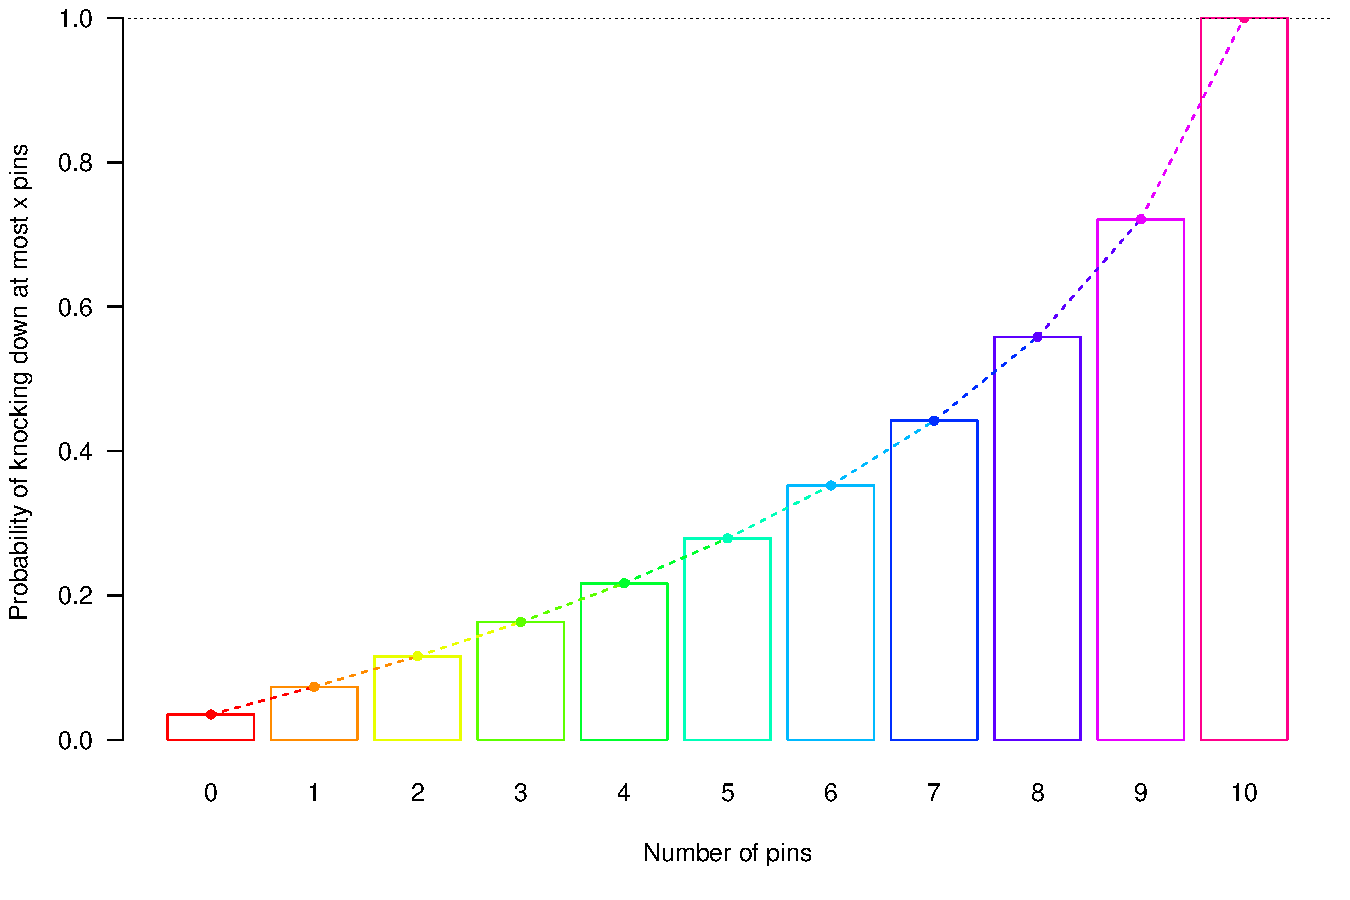
\includegraphics{Slides04_files/figure-beamer/unnamed-chunk-2-1.pdf}
\end{frame}

\begin{frame}{Cumulative Density Functions (CDFs)}
\protect\hypertarget{cumulative-density-functions-cdfs}{}
\begin{itemize}
\tightlist
\item
  Now \(\Omega\) is an interval; e.g.~\(\Omega=\mathbb{R}\),
  \(\Omega=\mathbb{R}_{+}\), \(\Omega=\left(a,b\right)\),
  \(\Omega=\left(0,1\right]\), etc.
\item
  \(\Omega\) has an infinite number of points with zero width, so
  \(\Pr\left(X = x\right) \downarrow 0\)
\item
  \(\Pr\left(X\leq x\right)\) is called the Cumulative Density Function
  (CDF) from \(\Omega\) to \(\left[0,1\right]\)
\item
  No conceptual difference between a CMF and a CDF except emphasis on
  whether \(\Omega\) is discrete or continuous so we use
  \(F\left(x \mid \boldsymbol{\theta}\right)\) for both
\end{itemize}
\end{frame}

\begin{frame}{From CDF to a Probability Density Function (PDF)}
\protect\hypertarget{from-cdf-to-a-probability-density-function-pdf}{}
\begin{itemize}[<+->]
\tightlist
\item
  \(\Pr\left(a<X\leq x\right)=F\left(x \mid \boldsymbol{\theta}\right)-F\left(a \mid \boldsymbol{\theta}\right)\)
  as in the discrete case
\item
  If \(x=a+h\),
  \(\frac{F\left(x \mid \boldsymbol{\theta}\right)-F\left(a \mid \boldsymbol{\theta}\right)}{x-a}=\frac{F\left(a+h \mid \boldsymbol{\theta}\right)-F\left(a \mid \boldsymbol{\theta}\right)}{h}\)
  is the slope of a line segment
\item
  If we then let \(h\downarrow0\),
  \(\frac{F\left(a+h \mid \boldsymbol{\theta}\right)-F\left(a \mid \boldsymbol{\theta}\right)}{h}\rightarrow\frac{\partial F\left(a \mid \boldsymbol{\theta}\right)}{\partial a}\equiv f\left(x \mid \boldsymbol{\theta}\right)\)
  is still the RATE OF CHANGE in
  \(F\left(x \mid \boldsymbol{\theta}\right)\) at \(x\), i.e. the slope
  of the CDF at \(x\)
\item
  The derivative of \(F\left(x\right)\) with respect to \(x\) is the
  Probability Density Function (PDF) \& denoted \(f\left(x\right)\),
  which is always positive because the CDF increases
\item
  \(f\left(x\right)\) is NOT a probability (it is a probability's slope)
  but is used like a PMF
\item
  Conversely,
  \(F\left(x\mid\theta\right) = \int_{-\infty}^x f\left(x \mid \theta\right)dx\)
  is the area under the PDF up to \(x\)
\item
  Can use WolframAlpha to take
  \href{https://www.wolframalpha.com/input/?i=partial+derivative}{derivatives}
  or do (some)
  \href{https://www.wolframalpha.com/input/?i=definite+integral}{definite
  integrals} but Columbia students can and should
  \href{https://cuit.columbia.edu/content/mathematica}{download} the
  full Mathematica for free. Also, you can do symbolic stuff in Python,
  whether \href{https://www.sympy.org/en/index.html}{locally} or
  \href{https://www.sympygamma.com/}{online}.
\end{itemize}
\end{frame}

\begin{frame}{Correspondence between Discrete \& Continuous}
\protect\hypertarget{correspondence-between-discrete-continuous}{}
\begin{longtable}[]{@{}
  >{\raggedright\arraybackslash}p{(\columnwidth - 6\tabcolsep) * \real{0.11}}
  >{\raggedright\arraybackslash}p{(\columnwidth - 6\tabcolsep) * \real{0.28}}
  >{\raggedright\arraybackslash}p{(\columnwidth - 6\tabcolsep) * \real{0.22}}
  >{\raggedright\arraybackslash}p{(\columnwidth - 6\tabcolsep) * \real{0.39}}@{}}
\toprule
\begin{minipage}[b]{\linewidth}\raggedright
Concept
\end{minipage} & \begin{minipage}[b]{\linewidth}\raggedright
Discrete \(X\) and \(Y\)
\end{minipage} & \begin{minipage}[b]{\linewidth}\raggedright
Continuous \(X\), \(Y\), and \(\theta\)
\end{minipage} & \begin{minipage}[b]{\linewidth}\raggedright
Comment
\end{minipage} \\
\midrule
\endhead
Cumulative &
\(F\left(x \mid \theta\right) = \Pr\left(X \leq x \mid \theta\right)\) &
\(F\left(x \mid \theta\right) = \Pr\left(X \leq x \mid \theta\right)\) &
CMF \& CDF are the same concept \\
Median & \(\arg\min_x:F\left(x \mid \theta\right) \geq \frac{1}{2}\) &
\(F^{-1}\left(\frac{1}{2} \mid \theta\right) = x\) &
\(F^{-1}\left(p\right)\) is an inverse CDF \\
Rate of Change &
\(\Pr\left(x \mid \theta \right) = \frac{F\left(x \mid \theta \right) - F\left(x - 1 \mid \theta\right)}{x - \left(x - 1\right)}\)
&
\(f\left(x \mid \theta\right) = \frac{\partial}{\partial x}F\left(x \mid \theta \right)\)
& \(f\) is a density, not a probability \\
Mode & \(\arg\max_x \Pr\left(x \mid \theta \right)\) &
\(\arg\max_x f\left(x \mid \theta\right)\) & Posterior mode is a red
herring \\
\(\mathbb{E}g\left(X \mid \theta\right)\) &
\(\sum_{x \in \Omega} g\left(x\right) \Pr\left(x \mid \theta\right)\) &
\(\int_{\Omega} g\left(x\right) f\left(x \mid \theta \right) dx\) &
Might not exist in continuous case \\
Mult. Rule &
\(\Pr\left(x \mid \theta \right) \Pr\left(y \mid x, \theta\right)\) &
\(f\left(x \mid \theta\right) f\left(y \mid x,\theta\right)\) &
Independence is a special case \\
Bayes Rule &
\(\frac{\Pr\left(x \bigcap y\right)}{\Pr\left(\bcancel{x} \bigcap y\right)} = \frac{\Pr\left(x\right) \Pr\left(y \mid x\right)}{\sum_{x \in \Omega} \Pr\left(x\right) \Pr\left(y \mid x\right)}\)
&
\(\frac{f\left(\theta \bigcap y\right)}{f\left(\bcancel{\theta} \bigcap y\right)} = \frac{f\left(\theta\right) f\left(y \mid \theta\right)}{\int_{-\infty}^\infty f\left(\theta\right) f\left(y \mid \theta\right)d\theta}\)
& But integrals are rarely elementary \\
\bottomrule
\end{longtable}
\end{frame}

\begin{frame}[fragile]{Uniform Distribution}
\protect\hypertarget{uniform-distribution}{}
\begin{itemize}
\tightlist
\item
  Standard uniform distribution for \(X \in \Omega = \left[0,1\right]\)
  with CDF \(F\left(x\right) = x\) and PDF \(f\left(x\right) = 1\), so
  the PDF is just a horizontal line at \(1\)
\item
  Can randomly draw from a standard uniform with
  \href{https://en.wikipedia.org/wiki/RDRAND}{hardware} but
  \texttt{runif} uses pseudo-random software emulation (conditional on
  \texttt{set.seed}) for speed
\item
  If \(\Omega = \left[a,b\right]\), CDF is
  \(F\left(x \mid a,b\right) = \frac{x - a}{b - a}\), PDF is
  \(f\left(x \mid, a,b\right) = \frac{1}{b - a}\), and draw is
  \texttt{a\ +\ (b\ -\ a)\ *\ runif(n\ =\ 1)} or
  \texttt{runif(n\ =\ 1,\ min\ =\ a,\ max\ =\ b)}
\item
  Let \(g\left(X\right) = -\ln f\left(x \mid a,b\right)\). The
  (differential) entropy of \(X\) is defined as
  \[\mathbb{E}g\left(X\right) = \int_a^b g\left(x\right) f\left(x \mid a, b\right) = 
  -\int_a^b \ln f\left(x \mid a,b\right) f\left(x \mid a,b\right) dx\]
  and is maximized for continuous RVs on \(\Omega = \left[a,b\right]\)
  by \(f\left(x \mid a,b\right) = \frac{1}{b - a}\). So, uniform
  distribution conveys no information about \(X\) beyond that
  \(\Omega = \left[a,b\right]\).
\end{itemize}
\end{frame}

\begin{frame}[fragile]{Exponential Distribution}
\protect\hypertarget{exponential-distribution}{}
\begin{itemize}
\tightlist
\item
  Can draw from the standard exponential distribution for
  \(X \in \Omega = \mathbb{R}_+\) by passing a standard uniform deviate,
  \(p\), through \(F^{-1}\left(p\right) = -\ln\left(1 - p\right) = x\)
\item
  \(F^{-1}\left(p\right)\) is called a quantile function from
  \(\left[0,1\right]\) to \(\Omega\), which can be inverted to obtain
  the CDF. In this case, \(F\left(x\right) = 1 - e^{-x} = p\) and thus
  \(f\left(x\right) = e^{-x}\).
\item
  To draw from a general exponential distribution with expectation
  \(\mu > 0\), do \texttt{mu\ *\ qexp(runif(n\ =\ 1))} or
  \texttt{rexp(n\ =\ 1,\ rate\ =\ 1\ /\ mu)}. In general,
  \(F^{-1}\left(p \mid \mu\right) = -\mu \ln \left(1 - p\right)\),
  \(F\left(x \mid \mu\right) = 1 - e^{-\frac{x}{\mu}}\),
  \(f\left(x \mid \mu\right) = \frac{1}{\mu}e^{-\frac{x}{\mu}}\),
  \[\mu = \mathbb{E}X = \int_0^\infty x \frac{1}{\mu} e^{-\frac{x}{\mu}} dx = 
  \left.-\left(x + \mu\right)e^{-\frac{x}{\mu}}\right|_0^\infty \rightarrow
  0 + \mu\]
\item
  Let \(g\left(X\right) = -\ln f\left(x \mid \mu\right)\). The
  (differential) entropy of \(X\) is defined as
  \(\mathbb{E}g\left(X \mid \mu\right)\) and is maximized for continuous
  RVs on \(\Omega = \mathbb{R}_+\) with \(\mathbb{E}X = \mu\) when
  \(f\left(x \mid \mu\right) = \frac{1}{\mu}e^{-\frac{x}{\mu}}\) is the
  exponential PDF.
\end{itemize}
\end{frame}

\begin{frame}{Plots for the Standard Exponential Distribution}
\protect\hypertarget{plots-for-the-standard-exponential-distribution}{}
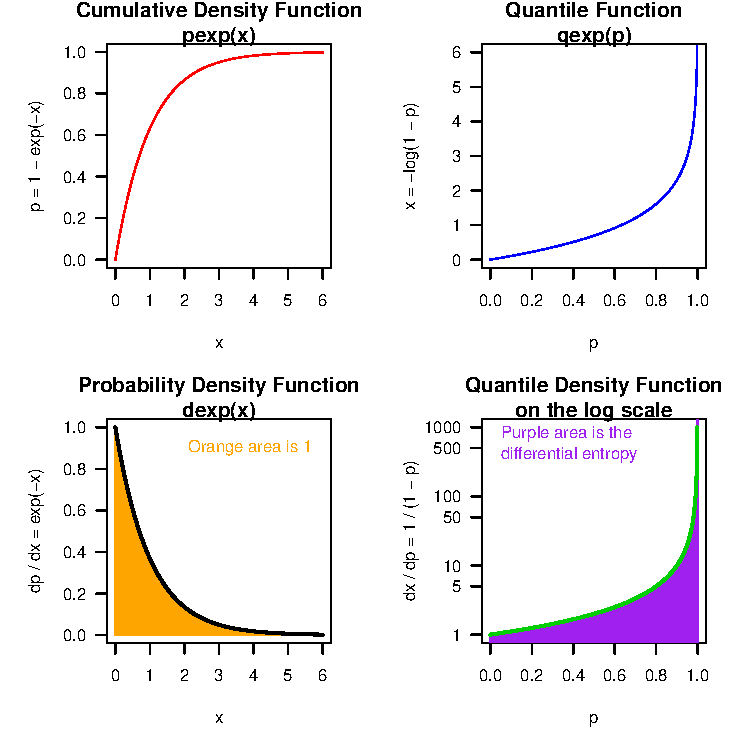
\includegraphics{Slides04_files/figure-beamer/unnamed-chunk-3-1.pdf}

\begin{itemize}
\tightlist
\item
  Functional forms are specific to the standard exponential distribution
  but relationships among concepts are general to all continuous RVs
\end{itemize}

\begin{itemize}[<+->]
\tightlist
\item
  Start with the top right plot. A simple algorithm to randomly draw
  from \(\Omega\) a realization of \(x\) is to draw \(p\) from a
  standard uniform, go up to the blue curve, and left to the vertical
  axis.
\item
  Flip the axes to go from blue to red
\item
  Red curve has a slope at every point and its slope is the black curve
\item
  Substitute \(F^{-1}\left(p\right)\) for \(x\) in black and take the
  reciprocal to get green
\end{itemize}
\end{frame}

\begin{frame}[fragile]{Standard Normal Distribution}
\protect\hypertarget{standard-normal-distribution}{}
\begin{itemize}
\tightlist
\item
  Let \(\phi\left(x\right) = \frac{e^{-\frac{1}{2}x^2}}{\sqrt{2\pi}}\)
  and
  \(\Phi\left(x\right) = \frac{1}{2} + \phi\left(x\right) \sum_{n = 0}^\infty \frac{x^{2n + 1}}{\left(2n + 1\right)!!}\),
  which involves the odd
  \href{https://en.wikipedia.org/wiki/Double_factorial}{double
  factorial} function, and
  \(F^{-1}\left(p\right) = x: \Phi\left(x\right) = p\) is implicit
\item
  The CDF for the standard normal distribution on
  \(\Omega = \mathbb{R}\) is \(F\left(x\right) = \Phi\left(x\right)\)
  and the PDF is
  \(f\left(x\right) = \phi\left(x\right) = \frac{\partial}{\partial x} \Phi\left(x\right)\),
  which can be shown fairly easily
\item
  Can draw from the standard normal distribution by passing a standard
  uniform variate, \(p\), through \(F^{-1}\left(p\right)\), which is
  implemented as \texttt{qnorm} in R
\end{itemize}

\begin{Shaded}
\begin{Highlighting}[]
\FunctionTok{c}\NormalTok{(}\FunctionTok{set.seed}\NormalTok{(}\DecValTok{20220214}\NormalTok{), }\AttributeTok{direct =} \FunctionTok{rnorm}\NormalTok{(}\DecValTok{1}\NormalTok{), }\FunctionTok{set.seed}\NormalTok{(}\DecValTok{20220214}\NormalTok{), }\AttributeTok{composed =} \FunctionTok{qnorm}\NormalTok{(}\FunctionTok{runif}\NormalTok{(}\DecValTok{1}\NormalTok{)))}
\end{Highlighting}
\end{Shaded}

\begin{verbatim}
##    direct  composed 
## 0.8441673 0.8441674
\end{verbatim}

\begin{itemize}
\tightlist
\item
  Since \(\phi\left(x\right)\) is an even function that only depends on
  \(x\) through \(x^2\), you can show that
  \(\mathbb{E}X = \int_{-\infty}^\infty x \phi\left(x\right) dx = \int_{-\infty}^0 x f\left(x\right) + \int_{0}^\infty x \phi\left(x\right) = 0\)
\end{itemize}
\end{frame}

\begin{frame}[fragile]{General (univariate) Normal Distribution}
\protect\hypertarget{general-univariate-normal-distribution}{}
\begin{itemize}
\tightlist
\item
  If \(Z\) is distributed standard normal, \(X = Z \sigma + \mu\) is
  distributed normal with expectation \(\mu\) and standard deviation
  \(\sigma > 0\)
\item
  Can draw from a normal distribution via
  \texttt{rnorm(n\ =\ 1,\ mu,\ sigma)} or, equivalently,
  \texttt{qnorm(runif(n\ =\ 1))\ *\ sigma\ +\ mu}
\item
  Let \(g\left(X\right) = -\ln f\left(x \mid \mu, \sigma\right)\). The
  (differential) entropy of \(X\) is defined as
  \(\mathbb{E}g\left(X \mid \mu, \sigma\right)\) and is maximized for
  continuous RVs on \(\Omega = \mathbb{R}\) with \(\mathbb{E}X = \mu\)
  and \(\mathbb{E}\left(X - \mu\right)^2 = \sigma^2\) when
  \(f\left(x \mid \mu, \sigma\right) = \frac{e^{-\frac{1}{2} \left(\frac{x - \mu}{\sigma}\right)^2}}{\sigma \sqrt{2 \pi}}\)
  is the normal PDF.
\item
  It may seem as if the normal distribution is very informative, but it
  conveys the least information beyond the fact that it is a real number
  with expectation \(\mu\) and standard deviation \(\sigma\). Thus, it
  is easy to move when conditioning on data.
\end{itemize}
\end{frame}

\begin{frame}{Different Parameterizations of a Distribution}
\protect\hypertarget{different-parameterizations-of-a-distribution}{}
\begin{itemize}
\tightlist
\item
  The normal PDF can be written in terms of an expectation, \(\mu\), and
  a STANDARD DEVIATION, \(\sigma\):
  \(f\left(x \mid \mu, \sigma\right) = \frac{e^{-\frac{1}{2}\left(\frac{x - \mu}{\sigma}\right)^2}}{\sigma\sqrt{2\pi}}\)
\item
  The normal PDF can be written in terms of an expectation, \(\mu\), and
  a VARIANCE, \(\nu = \sigma^2\):
  \(f\left(x \mid \mu, \nu\right) = \frac{e^{-\frac{1}{2\nu}\left(x - \mu\right)^2}}{\sqrt{2\pi\nu}}\)
\item
  The normal PDF can be written in terms of an expectation, \(\mu\), and
  a PRECISION, \(\tau = \frac{1}{\nu}\):
  \(f\left(x \mid \mu, \tau\right) = \frac{\sqrt{\tau} e^{-\frac{\tau}{2}\left(x - \mu\right)^2}}{\sqrt{2\pi}}\)
\item
  All three parameterizations imply the same things about \(X\). Using
  \(\sigma\) makes the most sense empirically because it is in the same
  units as \(X\). Using \(\nu\) is often convenient for proofs. Using
  \(\tau\) facilitated Bayesian computations before Stan was released in
  \(2011\) and is used in the Lancaster reading for next week.
\end{itemize}
\end{frame}

\begin{frame}{Bivariate Normal Distribution}
\protect\hypertarget{bivariate-normal-distribution}{}
If
\(\Pr\left(X \leq x \bigcap Y \leq y \mid \boldsymbol{\theta}\right) = F\left(x,y\mid\boldsymbol{\theta}\right)\)
is a biviariate CDF, then the bivariate PDF is
\(\frac{\partial^2}{\partial x \partial y}F\left(x,y\mid\boldsymbol{\theta}\right)\).
This also generalizes beyond two dimensions. The PDF of the bivariate
normal distribution over \(\Omega = \mathbb{R}^2\) has five parameters:
\[f\left(x,y\mid \mu_X,\mu_Y,\sigma_X,\sigma_Y,\rho\right) =\\
\frac{1}{2\pi\sigma_X\sigma_Y\sqrt{1-\rho^2}}e^{-\frac{1}{2\left(1-\rho^2\right)}
\left(\left(\frac{x - \mu_X}{\sigma_X}\right)^2 + 
\left(\frac{y - \mu_Y}{\sigma_Y}\right)^2 - 
2\rho\frac{x - \mu_X}{\sigma_X}\frac{y - \mu_Y}{\sigma_Y}\right)} = \\
\frac{1}{\sigma_X\sqrt{2\pi}}e^{-\frac{1}{2}\left(\frac{x - \mu_X}{\sigma_X}\right)^2} \times
\frac{1}{\color{blue}{\sigma_Y\sqrt{1-\rho^2}}\sqrt{2\pi}}e^{-\frac{1}{2}
\left(\frac{y - \left(\color{red}{\mu_Y + \frac{\sigma_Y}{\sigma_X}\rho\left(x-\mu_x\right)}\right)}
{\color{blue}{\sigma_Y\sqrt{1-\rho^2}}}\right)^2},\] where the first
term is a marginal normal PDF and the second is a conditional normal PDF
w/ parameters
\(\color{red}{\mu = \mu_Y + \frac{\sigma_Y}{\sigma_X}\rho\left(x-\mu_X\right)}\)
\& \(\color{blue}{\sigma = \sigma_Y\sqrt{1-\rho^2}}\).
\end{frame}

\begin{frame}[fragile]{Bivariate Normal PDF Visualized}
\protect\hypertarget{bivariate-normal-pdf-visualized}{}
\begin{Shaded}
\begin{Highlighting}[]
\NormalTok{dbinorm }\OtherTok{\textless{}{-}} \ControlFlowTok{function}\NormalTok{(x, y, }
                    \AttributeTok{mean\_x =} \DecValTok{5}\NormalTok{, }
                    \AttributeTok{mean\_y =} \DecValTok{5}\NormalTok{, }
                    \AttributeTok{sd\_x =} \FloatTok{1.5}\NormalTok{, }
                    \AttributeTok{sd\_y =} \FloatTok{1.0}\NormalTok{, }
                    \AttributeTok{rho =} \FloatTok{0.5}\NormalTok{) \{}
\NormalTok{  beta }\OtherTok{\textless{}{-}}\NormalTok{ rho }\SpecialCharTok{*}\NormalTok{ sd\_y }\SpecialCharTok{/}\NormalTok{ sd\_x}
\NormalTok{  mu\_yx }\OtherTok{\textless{}{-}}\NormalTok{ mean\_y }\SpecialCharTok{+}\NormalTok{ beta }\SpecialCharTok{*}\NormalTok{ (x }\SpecialCharTok{{-}}\NormalTok{ mean\_x)}
\NormalTok{  sigma\_yx }\OtherTok{\textless{}{-}}\NormalTok{ sd\_y }\SpecialCharTok{*} \FunctionTok{sqrt}\NormalTok{(}\DecValTok{1} \SpecialCharTok{{-}}\NormalTok{ rho }\SpecialCharTok{\^{}} \DecValTok{2}\NormalTok{)}
  \FunctionTok{return}\NormalTok{( }\FunctionTok{dnorm}\NormalTok{(x, mean\_x, sd\_x) }\SpecialCharTok{*} 
          \FunctionTok{dnorm}\NormalTok{(y, mu\_yx, sigma\_yx) )}
\NormalTok{\} }\CommentTok{\# does not come with R so define it}
\FunctionTok{library}\NormalTok{(rgl)}
\FunctionTok{persp3d}\NormalTok{(dbinorm, }\AttributeTok{xlim =} \FunctionTok{c}\NormalTok{(}\DecValTok{0}\NormalTok{, }\DecValTok{10}\NormalTok{), }
        \AttributeTok{ylim =} \FunctionTok{c}\NormalTok{(}\DecValTok{0}\NormalTok{, }\DecValTok{10}\NormalTok{), }\AttributeTok{axes =} \ConstantTok{FALSE}\NormalTok{,}
        \AttributeTok{alpha =} \FloatTok{0.75}\NormalTok{, }\AttributeTok{col =}\NormalTok{ rainbow,}
        \AttributeTok{zlab =} \StringTok{"density"}\NormalTok{)}
\FunctionTok{rglwidget}\NormalTok{()}
\end{Highlighting}
\end{Shaded}

\includegraphics{C:/Users/CINDYL~1/AppData/Local/Temp/RtmpQz9A7t/file29ac19a922.png}
\end{frame}

\begin{frame}[fragile]{Bayes Rule with Normal Distributions}
\protect\hypertarget{bayes-rule-with-normal-distributions}{}
\begin{itemize}
\tightlist
\item
  Suppose \(X\) and \(Y\) are distributed bivariate normal with
  parameters \(\mu_X,\mu_Y,\sigma_X,\sigma_Y\) and \(\rho\). Thus,
  \[f\left(x \mid y, \mu_X,\mu_Y,\sigma_X,\sigma_Y, \rho \right) = 
  \frac{f_X\left(x \mid \mu_X, \sigma_X\right) 
  f_{Y\mid X}\left(y \mid \color{red}{\mu_Y + \frac{\sigma_Y}{\sigma_X}\rho\left(x-\mu_X\right)}, 
  \color{blue}{\sigma_Y\sqrt{1 - \rho^2}}\right)}
  {f\left(\bcancel{x}, y \mid\mu_X,\mu_Y,\sigma_X,\sigma_Y,\rho\right)}\]
  and the marginal PDF of \(Y\) is univariate normal (by interchanging
  \(X\) w/ \(Y\) on the previous slides) since
  \[f\left(\bcancel{x}, y \mid\mu_X,\mu_Y,\sigma_X,\sigma_Y,\rho\right) =
  \int_{-\infty}^\infty f\left(x, y \mid\mu_X,\mu_Y,\sigma_X,\sigma_Y,\rho\right) dx =
  \frac{e^{-\frac{1}{2}\left(\frac{y - \mu_Y}{\sigma_Y}\right)^2}}{\sigma_Y \sqrt{2 \pi}} = 
  f_Y\left(y \mid \mu_Y, \sigma_Y\right)\]
\item
  In this very rare case, marginalization can be done analytically, but
  the area can also be obtained via:
\end{itemize}

\begin{Shaded}
\begin{Highlighting}[]
\NormalTok{mu\_X }\OtherTok{\textless{}{-}} \FloatTok{9.8}\NormalTok{; sigma\_X }\OtherTok{\textless{}{-}} \FloatTok{7.6}\NormalTok{; mu\_Y }\OtherTok{\textless{}{-}} \FloatTok{5.4}\NormalTok{; sigma\_Y }\OtherTok{\textless{}{-}} \FloatTok{3.2}\NormalTok{; rho }\OtherTok{\textless{}{-}} \SpecialCharTok{{-}}\FloatTok{0.1}\NormalTok{; y }\OtherTok{\textless{}{-}} \FunctionTok{sqrt}\NormalTok{(}\DecValTok{5}\NormalTok{)}
\NormalTok{denominator }\OtherTok{\textless{}{-}} \FunctionTok{integrate}\NormalTok{(dbinorm, }\AttributeTok{lower =} \SpecialCharTok{{-}}\ConstantTok{Inf}\NormalTok{, }\AttributeTok{upper =} \ConstantTok{Inf}\NormalTok{, }\AttributeTok{y =}\NormalTok{ y, }\CommentTok{\# uses little trapezoids basically}
                         \AttributeTok{mean\_x =}\NormalTok{ mu\_X, }\AttributeTok{mean\_y =}\NormalTok{ mu\_Y, }\AttributeTok{sd\_x =}\NormalTok{ sigma\_X, }\AttributeTok{sd\_y =}\NormalTok{ sigma\_Y, }\AttributeTok{rho =}\NormalTok{ rho)}\SpecialCharTok{$}\NormalTok{value}
\FunctionTok{format}\NormalTok{(}\FunctionTok{c}\NormalTok{(}\AttributeTok{exact =} \FunctionTok{dnorm}\NormalTok{(y, }\AttributeTok{mean =}\NormalTok{ mu\_Y, }\AttributeTok{sd =}\NormalTok{ sigma\_Y), }\AttributeTok{numeric =}\NormalTok{ denominator), }\AttributeTok{digits =} \DecValTok{10}\NormalTok{)}
\end{Highlighting}
\end{Shaded}

\begin{verbatim}
##           exact         numeric 
## "0.07646809985" "0.07646809983"
\end{verbatim}
\end{frame}

\begin{frame}[fragile]{Biontech / Pfizer
\href{http://skranz.github.io//r/2020/11/11/CovidVaccineBayesian.html}{Analysis}
of First Covid Vaccine}
\protect\hypertarget{biontech-pfizer-analysis-of-first-covid-vaccine}{}
\begin{itemize}
\tightlist
\item
  Let \(\pi_v\) be the probability of getting covid given that someone
  is vaccinated (in the Fall of 2020), \(\pi_c\) be the probability of
  getting covid given that someone is not vaccinated,
  \(\theta = \frac{\pi_v}{\pi_v + \pi_c}\), and the ``Vaccine Effect''
  is
  \(\mbox{VE}\left(\theta\right) = \frac{1 - 2\theta}{1 - \theta} \leq 1\)
\item
  Beta distribution has PDF
  \(f\left(\theta \mid a,b\right) = \frac{\theta^{a - 1}\left(1 - \theta\right)^{b - 1}} {\int_0^1 t^{a - 1}\left(1 - t\right)^{b - 1}dt} = \frac{\theta^{a - 1}\left(1 - \theta\right)^{b - 1}}{B\left(a,b\right)}\)
\item
  Prior for \(\theta\) was Beta with \(a = 0.700102\) and \(b = 1\),
  which was chosen (poorly) so that the VE at
  \(\mathbb{E}\theta = \frac{a}{a + b}\) was about \(0.3\) (but it
  mattered little)
\end{itemize}

\begin{Shaded}
\begin{Highlighting}[]
\FunctionTok{library}\NormalTok{(dplyr)}
\FunctionTok{library}\NormalTok{(ggplot2)}
\NormalTok{a }\OtherTok{\textless{}{-}} \FloatTok{0.700102} 
\NormalTok{b }\OtherTok{\textless{}{-}} \DecValTok{1}
\FunctionTok{ggplot}\NormalTok{(}\FunctionTok{tibble}\NormalTok{(}\AttributeTok{theta =} \FunctionTok{rbeta}\NormalTok{(}\AttributeTok{n =} \DecValTok{10}\SpecialCharTok{\^{}}\DecValTok{6}\NormalTok{, }\AttributeTok{shape1 =}\NormalTok{ a, }\AttributeTok{shape2 =}\NormalTok{ b),}
              \AttributeTok{VE =}\NormalTok{ (}\DecValTok{1} \SpecialCharTok{{-}} \DecValTok{2} \SpecialCharTok{*}\NormalTok{ theta) }\SpecialCharTok{/}\NormalTok{ (}\DecValTok{1} \SpecialCharTok{{-}}\NormalTok{ theta))) }\SpecialCharTok{+} 
  \FunctionTok{geom\_density}\NormalTok{(}\FunctionTok{aes}\NormalTok{(}\AttributeTok{x =}\NormalTok{ VE)) }\SpecialCharTok{+} \FunctionTok{xlim}\NormalTok{(}\SpecialCharTok{{-}}\DecValTok{5}\NormalTok{, }\DecValTok{1}\NormalTok{) }\CommentTok{\# see next slide}
\end{Highlighting}
\end{Shaded}

\begin{verbatim}
## Warning: Removed 102105 rows containing non-finite values (stat_density).
\end{verbatim}
\end{frame}

\begin{frame}{Implied Prior Distribution of
\(\mbox{VE}\left(\theta\right)\)}
\protect\hypertarget{implied-prior-distribution-of-mboxveleftthetaright}{}
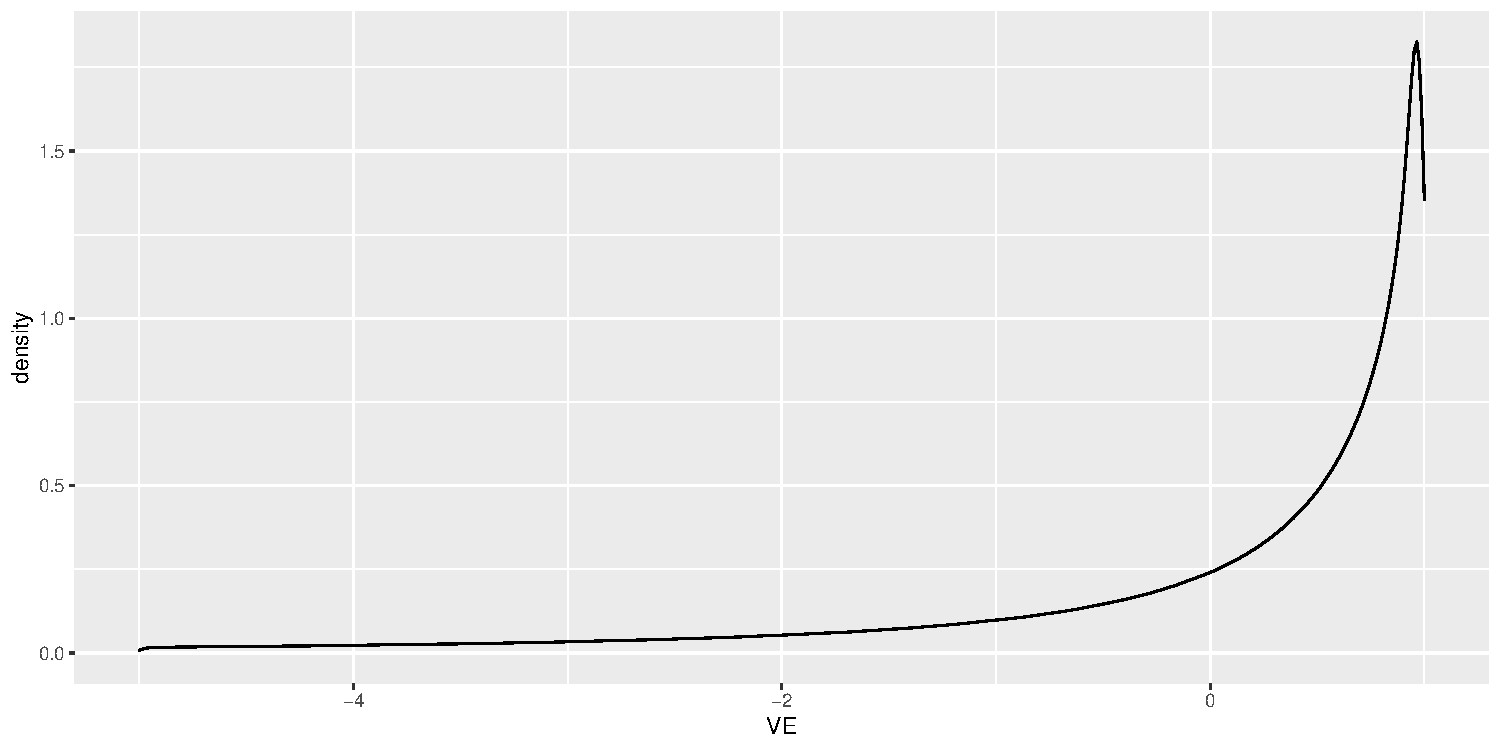
\includegraphics{Slides04_files/figure-beamer/prior-1.pdf}
\end{frame}

\begin{frame}{Deriving a Posterior Distribution of \(\theta\)
Analytically}
\protect\hypertarget{deriving-a-posterior-distribution-of-theta-analytically}{}
\begin{itemize}
\tightlist
\item
  \(\Pr\left(y \mid \theta, n\right) = {n \choose y} \theta^y \left(1 - \theta\right)^{n - y}\)
  is binomial given \(\theta\), where ``success'' is getting covid when
  vaccinated and ``failure'' is getting covid when unvaccinated
\item
  \(y = 8\) vaccinated people and \(n - y = 86\) non-vaccinated people
  got covid
\end{itemize}

\begin{itemize}[<+->]
\tightlist
\item
  What are their beliefs about \(\theta\)? (\(\propto\) means
  ``proportional to'', i.e.~the kernel)
  \[f\left(\theta \mid a,b,n,y\right) = \frac{f\left(\theta \mid a,b\right) L\left(\theta;n,y\right)}
  {\int_0^1 f\left(\theta \mid a,b\right) L\left(\theta;n,y\right) d\theta} \propto \\
  \theta^{a - 1} \left(1 - \theta\right)^{b - 1} \theta^{y}\left(1-\theta\right)^{n-y}
  = \theta^{a + y - 1} \left(1 - \theta\right)^{b + n - y - 1} = \theta^{a^\ast - 1} \left(1 - \theta\right)^{b^\ast - 1}\]
  where \(a^{\ast}=a+y = 8.700102\) and \(b^{\ast}=b+n-y = 87\)
\item
  \(f\left(\theta \mid a^\ast,b^\ast\right)\) has the kernel of a Beta
  PDF and therefore its normalizing constant must be the reciprocal of
  \(B\left(a^\ast,b^\ast\right) = \int_0^1 t^{a^\ast - 1} \left(1 - t\right)^{b^\ast - 1} dt\)
\end{itemize}
\end{frame}

\begin{frame}[fragile]{Implied Posterior Distribution of
\(\mbox{VE}\left(\theta\right)\)}
\protect\hypertarget{implied-posterior-distribution-of-mboxveleftthetaright}{}
\begin{Shaded}
\begin{Highlighting}[]
\NormalTok{y }\OtherTok{\textless{}{-}} \DecValTok{8}\NormalTok{; n }\OtherTok{\textless{}{-}} \DecValTok{94}\NormalTok{; a\_star }\OtherTok{\textless{}{-}}\NormalTok{ a }\SpecialCharTok{+}\NormalTok{ y; b\_star }\OtherTok{\textless{}{-}}\NormalTok{ b }\SpecialCharTok{+}\NormalTok{ n }\SpecialCharTok{{-}}\NormalTok{ y}
\FunctionTok{ggplot}\NormalTok{(}\FunctionTok{tibble}\NormalTok{(}\AttributeTok{theta =} \FunctionTok{rbeta}\NormalTok{(}\AttributeTok{n =} \DecValTok{10}\SpecialCharTok{\^{}}\DecValTok{6}\NormalTok{, }\AttributeTok{shape1 =}\NormalTok{ a\_star, }\AttributeTok{shape2 =}\NormalTok{ b\_star),}
              \AttributeTok{VE =}\NormalTok{ (}\DecValTok{1} \SpecialCharTok{{-}} \DecValTok{2} \SpecialCharTok{*}\NormalTok{ theta) }\SpecialCharTok{/}\NormalTok{ (}\DecValTok{1} \SpecialCharTok{{-}}\NormalTok{ theta))) }\SpecialCharTok{+} \FunctionTok{geom\_density}\NormalTok{(}\FunctionTok{aes}\NormalTok{(}\AttributeTok{x =}\NormalTok{ VE))}
\end{Highlighting}
\end{Shaded}

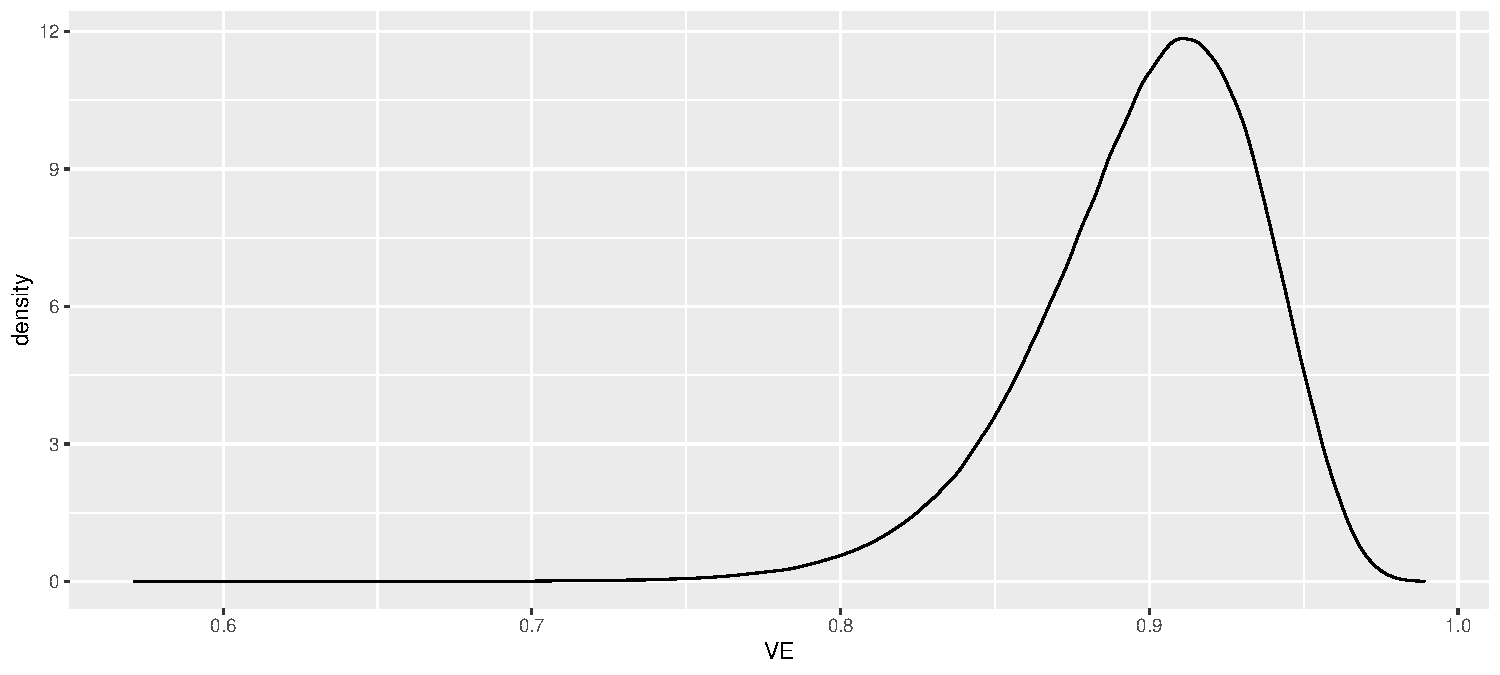
\includegraphics{Slides04_files/figure-beamer/unnamed-chunk-8-1.pdf}
\end{frame}

\begin{frame}[fragile]{Bowling with a Continuous Inability Parameter}
\protect\hypertarget{bowling-with-a-continuous-inability-parameter}{}
\begin{itemize}
\tightlist
\item
  Last week, we used
  \(\Pr\left(x \mid n, \Upsilon\right) = \frac{\log_{n + 2 + \Upsilon}\left(1 + \frac{1}{n + 1 + \Upsilon - x}\right)}{1 - \log_{n + 2 + \Upsilon}\left(1 + \Upsilon\right)}\)
  but this does not actually require that \(\Upsilon\) be a non-negative
  integer
\item
  Substitute \(1 + \Upsilon = \theta\) where \(\theta \geq 0\) is
  continuous
\item
  We can work backward from \(\mathbb{E}X_1 \mid \theta\) to a prior for
  \(\theta\)
\end{itemize}

\begin{Shaded}
\begin{Highlighting}[]
\FunctionTok{library}\NormalTok{(scales)}
\NormalTok{E }\OtherTok{\textless{}{-}} \ControlFlowTok{function}\NormalTok{(theta) }\FunctionTok{sapply}\NormalTok{(theta, }\AttributeTok{FUN =} \ControlFlowTok{function}\NormalTok{(t) }\FunctionTok{sum}\NormalTok{(Omega }\SpecialCharTok{*} \FunctionTok{Pr}\NormalTok{(Omega, }\AttributeTok{n =} \DecValTok{10}\NormalTok{, t)))}
\FunctionTok{ggplot}\NormalTok{() }\SpecialCharTok{+} \CommentTok{\# Pr(x, n = 10, theta = 1) and Omega were defined above by source("bowling.R")}
  \FunctionTok{geom\_function}\NormalTok{(}\AttributeTok{fun =} \SpecialCharTok{\textasciitilde{}}\FunctionTok{E}\NormalTok{(.x)) }\SpecialCharTok{+} \CommentTok{\# see next slide}
  \FunctionTok{scale\_x\_continuous}\NormalTok{(}\AttributeTok{limits =} \FunctionTok{c}\NormalTok{(}\FloatTok{1e{-}16}\NormalTok{, }\DecValTok{11000}\NormalTok{), }\AttributeTok{trans  =} \StringTok{"log10"}\NormalTok{,}
                     \AttributeTok{breaks =} \FunctionTok{trans\_breaks}\NormalTok{(}\StringTok{"log10"}\NormalTok{, }\ControlFlowTok{function}\NormalTok{(x) }\DecValTok{10}\SpecialCharTok{\^{}}\NormalTok{x),}
                     \AttributeTok{labels =} \FunctionTok{trans\_format}\NormalTok{(}\StringTok{"log10"}\NormalTok{, }\FunctionTok{math\_format}\NormalTok{(}\DecValTok{10}\SpecialCharTok{\^{}}\NormalTok{.x))) }\SpecialCharTok{+}
  \FunctionTok{ylab}\NormalTok{(}\StringTok{"Conditional expectation of first roll given theta"}\NormalTok{) }\SpecialCharTok{+}
  \FunctionTok{xlab}\NormalTok{(}\StringTok{"theta (log scale)"}\NormalTok{)}
\end{Highlighting}
\end{Shaded}
\end{frame}

\begin{frame}{Plot from Previous Slide}
\protect\hypertarget{plot-from-previous-slide}{}
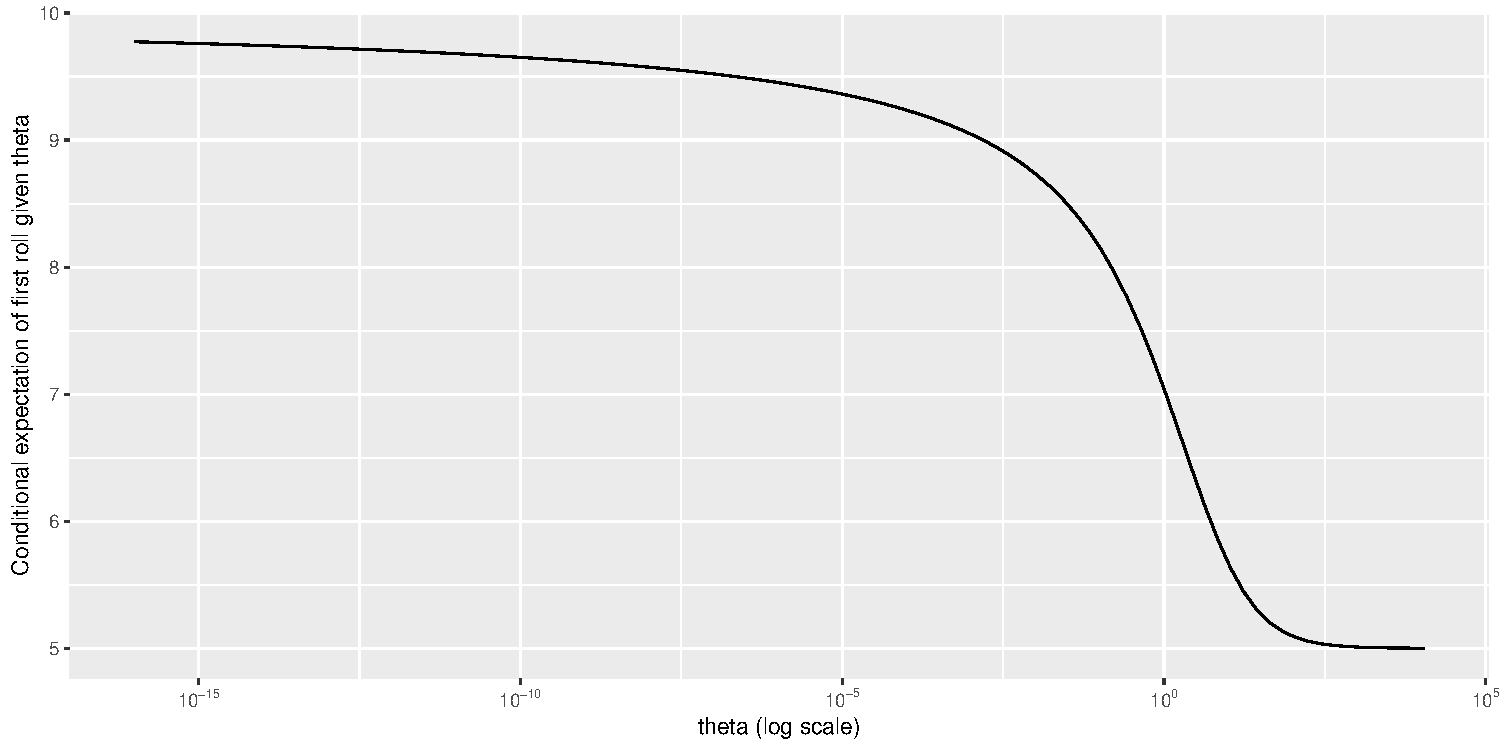
\includegraphics{Slides04_files/figure-beamer/unnamed-chunk-10-1.pdf}
\end{frame}

\begin{frame}{Marginal Probability of the First Roll in Bowling}
\protect\hypertarget{marginal-probability-of-the-first-roll-in-bowling}{}
\begin{itemize}
\tightlist
\item
  Suppose we utilize a standard exponential prior for \(\theta\), which
  has the MARGINAL PDF \(f\left(\theta\right) = e^{-\theta}\) and
  expectation \(\mu = 1\)
\item
  The CONDITIONAL PMF of \(X_1 \mid \theta\) is
  \(\Pr\left(x_1 \mid n, \theta\right) = \frac{\log_{n + 1 + \theta}\left(1 + \frac{1} {n + \theta - x_1}\right)}{1 - \log_{n + 1 + \theta}\left(\theta\right)}\)
\item
  The BIVARIATE PDF of \(\theta\) and \(X_1\) is
  \(f\left(\theta, x_1 \mid n\right) = e^{-\theta} \frac{\log_{n + 1 + \theta}\left(1 + \frac{1}{n + \theta - x_1}\right)}{1 - \log_{n + 1 + \theta}\left(\theta\right)}\)
\item
  The MARGINAL PMF of \(X_1\) is
  \[\Pr\left(x_1 \mid n\right) = f\left(\bcancel{\theta}, x_1 \mid n\right) = 
  \int_0^\infty e^{-\theta} \frac{\log_{n + 1 + \theta}\left(1 + \frac{1}{n + \theta - x_1}\right)}
  {1 - \log_{n + 1 + \theta}\left(\theta\right)}d\theta\] but we can't
  obtain the antiderivative to evalute the area
\end{itemize}

\begin{itemize}[<+->]
\tightlist
\item
  The \href{https://en.wikipedia.org/wiki/Risch_algorithm}{Risch
  algorithm} can tell you if a function has an elementary antiderivative
\end{itemize}
\end{frame}

\begin{frame}[fragile]{Marginalized Probability of the First Roll}
\protect\hypertarget{marginalized-probability-of-the-first-roll}{}
\begin{Shaded}
\begin{Highlighting}[]
\NormalTok{joint }\OtherTok{\textless{}{-}} \ControlFlowTok{function}\NormalTok{(theta, x\_1) }\FunctionTok{dexp}\NormalTok{(theta) }\SpecialCharTok{*} \FunctionTok{sapply}\NormalTok{(theta, }\AttributeTok{FUN =}\NormalTok{ Pr, }\AttributeTok{x =}\NormalTok{ x\_1, }\AttributeTok{n =} \DecValTok{10}\NormalTok{)}
\end{Highlighting}
\end{Shaded}

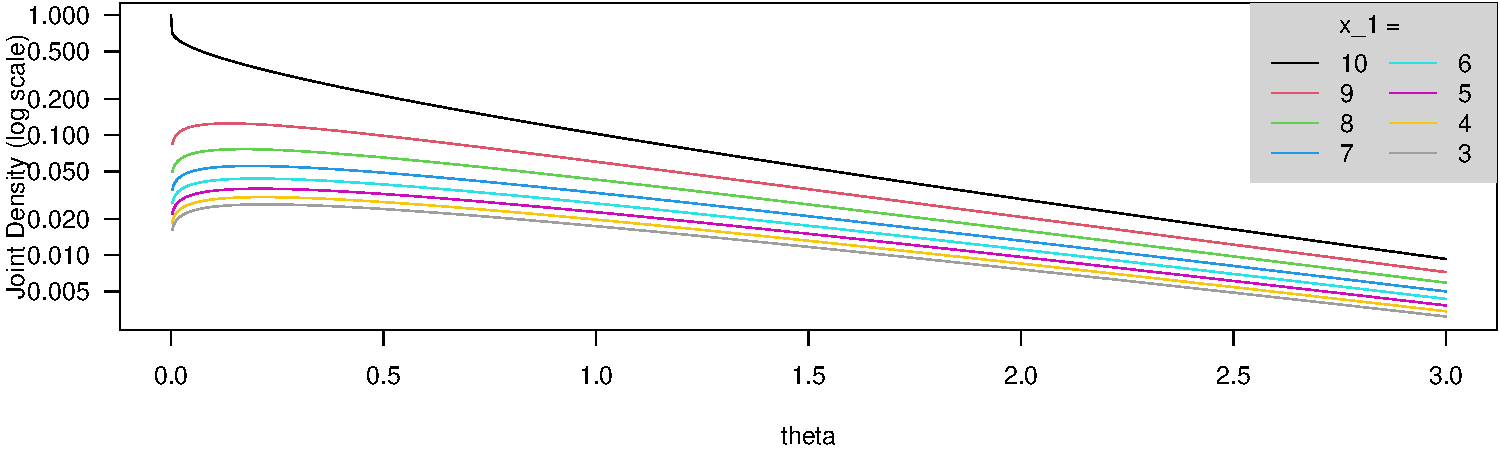
\includegraphics{Slides04_files/figure-beamer/unnamed-chunk-12-1.pdf}

\begin{Shaded}
\begin{Highlighting}[]
\NormalTok{marginal }\OtherTok{\textless{}{-}} \FunctionTok{integrate}\NormalTok{(joint, }\AttributeTok{lower =} \DecValTok{0}\NormalTok{, }\AttributeTok{upper =} \ConstantTok{Inf}\NormalTok{, }\AttributeTok{x\_1 =} \DecValTok{8}\NormalTok{)}\SpecialCharTok{$}\NormalTok{value}
\NormalTok{marginal}
\end{Highlighting}
\end{Shaded}

\begin{verbatim}
## [1] 0.1059296
\end{verbatim}
\end{frame}

\begin{frame}[fragile]{Deterministic Posterior PDF Given \(x_1 = 8\)}
\protect\hypertarget{deterministic-posterior-pdf-given-x_1-8}{}
\begin{Shaded}
\begin{Highlighting}[]
\NormalTok{E }\OtherTok{\textless{}{-}} \FunctionTok{integrate}\NormalTok{(}\ControlFlowTok{function}\NormalTok{(t) t }\SpecialCharTok{*} \FunctionTok{joint}\NormalTok{(t, }\AttributeTok{x =} \DecValTok{8}\NormalTok{) }\SpecialCharTok{/}\NormalTok{ marginal, }\AttributeTok{lower =} \DecValTok{0}\NormalTok{, }\AttributeTok{upper =} \ConstantTok{Inf}\NormalTok{)}\SpecialCharTok{$}\NormalTok{value}
\FunctionTok{ggplot}\NormalTok{() }\SpecialCharTok{+} \FunctionTok{xlim}\NormalTok{(}\DecValTok{0}\NormalTok{, }\DecValTok{5}\NormalTok{) }\SpecialCharTok{+} \FunctionTok{xlab}\NormalTok{(}\StringTok{"theta"}\NormalTok{) }\SpecialCharTok{+} \FunctionTok{ylab}\NormalTok{(}\StringTok{"Density"}\NormalTok{) }\SpecialCharTok{+} 
  \FunctionTok{geom\_function}\NormalTok{(}\AttributeTok{fun =} \SpecialCharTok{\textasciitilde{}}\FunctionTok{dexp}\NormalTok{(.x), }\AttributeTok{color =} \StringTok{"blue"}\NormalTok{) }\SpecialCharTok{+} \CommentTok{\# prior PDF}
  \FunctionTok{geom\_function}\NormalTok{(}\AttributeTok{fun =} \SpecialCharTok{\textasciitilde{}}\FunctionTok{joint}\NormalTok{(.x, }\AttributeTok{x =} \DecValTok{8}\NormalTok{) }\SpecialCharTok{/}\NormalTok{ marginal, }\AttributeTok{color =} \StringTok{"black"}\NormalTok{) }\SpecialCharTok{+} \CommentTok{\# posterior PDF}
  \FunctionTok{geom\_vline}\NormalTok{(}\FunctionTok{aes}\NormalTok{(}\AttributeTok{xintercept =}\NormalTok{ E), }\AttributeTok{color =} \StringTok{"red"}\NormalTok{) }\CommentTok{\# posterior expectation}
\end{Highlighting}
\end{Shaded}

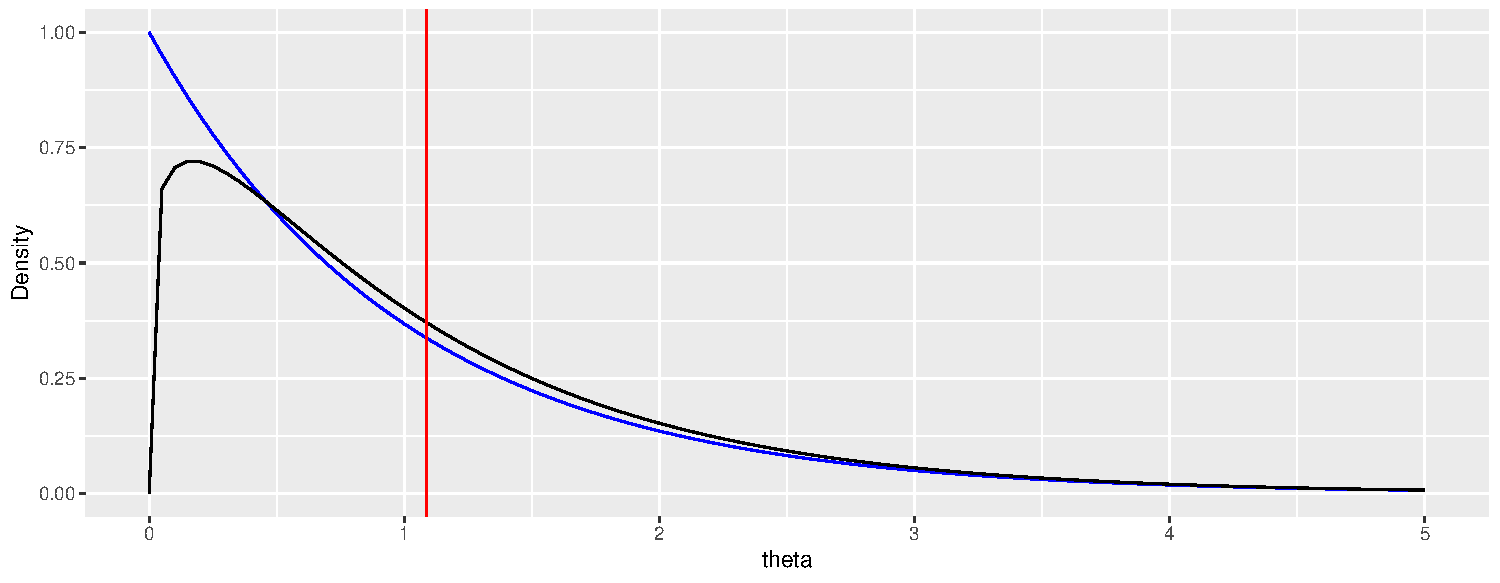
\includegraphics{Slides04_files/figure-beamer/unnamed-chunk-14-1.pdf}
\end{frame}

\begin{frame}[fragile]{Simulated Posterior Distribution Given
\(x_1 = 8\)}
\protect\hypertarget{simulated-posterior-distribution-given-x_1-8}{}
\begin{Shaded}
\begin{Highlighting}[]
\FunctionTok{tibble}\NormalTok{(}\AttributeTok{theta =} \FunctionTok{rexp}\NormalTok{(}\AttributeTok{n =} \DecValTok{10}\SpecialCharTok{\^{}}\DecValTok{6}\NormalTok{)) }\SpecialCharTok{\%\textgreater{}\%} \CommentTok{\# "infinite" draws from standard exponential prior}
  \FunctionTok{filter}\NormalTok{(}\DecValTok{8} \SpecialCharTok{==} \FunctionTok{vapply}\NormalTok{(theta, }\AttributeTok{FUN.VALUE =} \FunctionTok{integer}\NormalTok{(}\DecValTok{1}\NormalTok{), }\AttributeTok{FUN =} \ControlFlowTok{function}\NormalTok{(t) }
    \FunctionTok{sample}\NormalTok{(Omega, }\AttributeTok{size =} \DecValTok{1}\NormalTok{, }\AttributeTok{prob =} \FunctionTok{Pr}\NormalTok{(Omega, }\AttributeTok{n =} \DecValTok{10}\NormalTok{, t)))) }\SpecialCharTok{\%\textgreater{}\%}
  \FunctionTok{ggplot}\NormalTok{() }\SpecialCharTok{+} \FunctionTok{xlim}\NormalTok{(}\DecValTok{0}\NormalTok{, }\DecValTok{5}\NormalTok{) }\SpecialCharTok{+} \FunctionTok{xlab}\NormalTok{(}\StringTok{"theta"}\NormalTok{) }\SpecialCharTok{+} \FunctionTok{ylab}\NormalTok{(}\StringTok{"Density"}\NormalTok{) }\SpecialCharTok{+} 
  \FunctionTok{geom\_function}\NormalTok{(}\AttributeTok{fun =} \SpecialCharTok{\textasciitilde{}}\FunctionTok{dexp}\NormalTok{(.x), }\AttributeTok{color =} \StringTok{"blue"}\NormalTok{) }\SpecialCharTok{+} \CommentTok{\# prior PDF (exact)}
  \FunctionTok{geom\_density}\NormalTok{(}\FunctionTok{aes}\NormalTok{(}\AttributeTok{x =}\NormalTok{ theta), }\AttributeTok{color =} \StringTok{"black"}\NormalTok{)  }\SpecialCharTok{+} \CommentTok{\# posterior PDF (approximate)}
  \FunctionTok{geom\_vline}\NormalTok{(}\FunctionTok{aes}\NormalTok{(}\AttributeTok{xintercept =} \FunctionTok{mean}\NormalTok{(theta)), }\AttributeTok{color =} \StringTok{"red"}\NormalTok{) }\CommentTok{\# posterior mean (approximate)}
\end{Highlighting}
\end{Shaded}

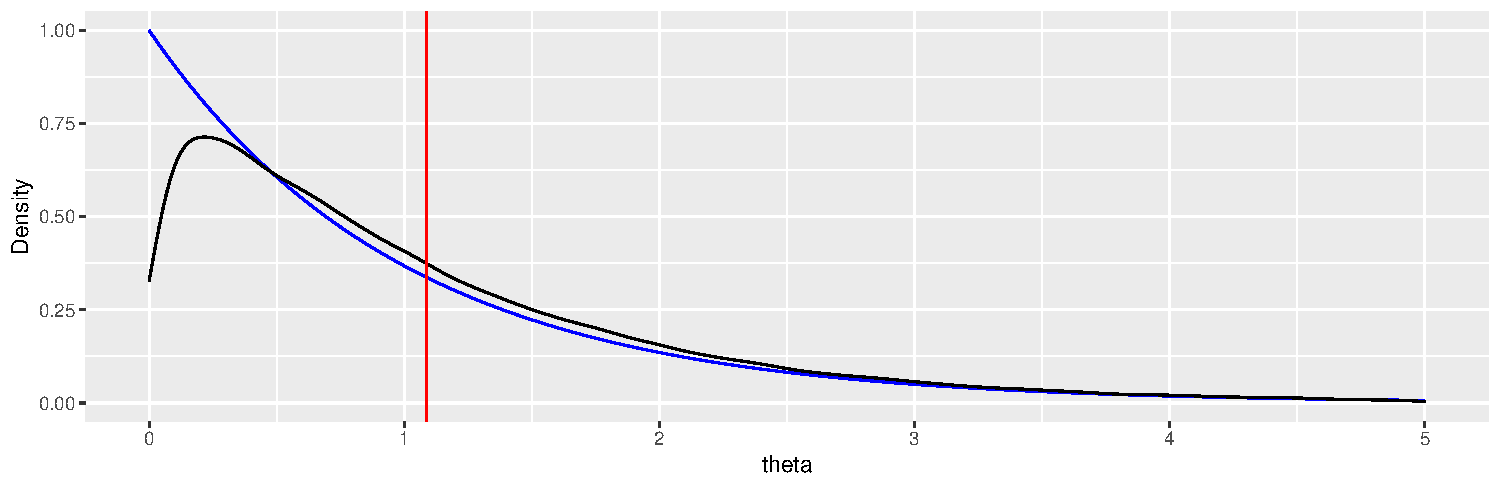
\includegraphics{Slides04_files/figure-beamer/sim-1.pdf}
\end{frame}

\end{document}
